\documentclass{abntex2}
\usepackage[brazil]{babel}
\usepackage[utf8]{inputenc}
\usepackage{indentfirst}
\usepackage{microtype}
%\usepackage{lmodern}
\usepackage{mathptmx} % Define a fonte Times para texto e matemática
\usepackage{amsmath}
\usepackage{amssymb}
\usepackage{graphicx}
\usepackage{subfig}
\usepackage[num]{abntex2cite}
\usepackage{hyperref}
\usepackage{fancyhdr}
\usepackage{siunitx}

\begin{document}

\begin{figure}[h]
    \centering
    
\includegraphics[width=0.5\linewidth]{vestibular-puc-goias-2021-2.jpg}
\end{figure}

\vspace{1cm}

\begin{center}
    {\huge Resolução de Circuito Elétrico com\\ Equação Diferencial de Segunda Ordem}\\
    \vspace{0.1cm}
    {Lucas Pereira Nunes}\\
    {9 de Novembro de 2024}\\
\end{center}

\vspace{5cm}

\begin{center}
            \Large{PONTIFÍCIA UNIVERSIDADE CATÓLICA DE GOIÁS\\
ESCOLA POLITÉCNICA E DE ARTES}

\vspace{4.2cm}
{\large Professor: Cristian Patricio Novoa Bustos}

\vfill
{GOIÂNIA - GO}
    \end{center}

\newpage
\textual
\setcounter{page}{1}

\section*{\textbf{Enunciado:\\}}

\begin{figure}[h]
    \centering
    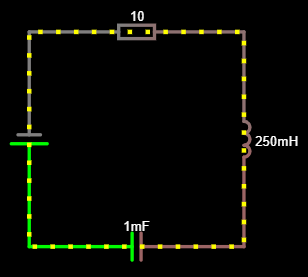
\includegraphics[width=0.5\linewidth]{image.png}
    \caption{Figura ilustrativa do circuito}
    \label{fig:enter-label}
\end{figure}

\subsection*{\Large Ache a carga $q(t)$ e a corrente $i(t)$ quando $E(t) = E_0\sin{{\alpha}t}$ e $L = 0,25H$, $R = \SI{10}{\ohm}$, $C = 0,001F$, $q(0) = q_0$, $i(0) = i_0$.}

\vspace{1.5cm}
\section*{\textbf{Resolução:}}
\subsection*{\Large Primeiramente, iremos modelar a EDO e substituir os números decimais por frações, \\considerando que o circuito pode ser modelado da seguinte maneira: $Lq'' + Rq' + \frac{1}{C}q = E(t)$, então:}
\begin{equation*}
    \frac{1}{4}q'' + 10q' + 1000q = E_0\sin{{\alpha}t}\\
\end{equation*}
\\
\Large Multiplicando a equação por 4:\\
\begin{equation*}
    q'' + 40q' + 4000q = 4E_0\sin{{\alpha}t}
\end{equation*}

\newpage
\Large Agora iremos resolver a parte homogênea da equação:\\
\begin{eqnarray*}
    m^2 + 40m + 4000 = 0\\
    \Delta = 1600 - 16000 = -14400\\
    \sqrt{\Delta} = 120i\\
    m = \frac{-40\pm120i}{2} = -20\pm60i\\
    \therefore \alpha = -20, \beta = 60
\end{eqnarray*}

\Large Uma vez que possuimos os valores de $\alpha$ e $\beta$ podemos montar a solução geral levando em conta que: $q_h = e^{{\alpha}t} (C_1 \cos{\beta t} + C_2 \sin{\beta t})$, então:\\
\begin{equation*}
    q_h = e^{-20t} (C_1 \cos{60t} + C_2 \sin{60t})
\end{equation*}
\Large Esta é nossa parte homogênea.
\vspace{0.5cm}

Agora iremos calcular o Wronskiano da Equação para que possamos começar a trabalhar na parte particular.
\vspace{0.5cm}
Podemos calcular o Wronskiano pela seguinte maneira:
$$ W(q_1, ..., q_n)=\left(\begin{array}{cccc}
q_{1} & q_{2} & \cdots & q_{n}\\
q'_{1} & q'_{2} & \cdots & q'_{n}\\
\vdots & \vdots & \ddots & \vdots\\
q^{(n-1)}_{1} & q^{(n-1)}_{2} & \cdots & q^{(n-1)}_{n}
\end{array}\right) $$
\\
\Large Sendo $q_1 = e^{-20t}\cos{60t}$ e $q_2 = e^{-20t}\sin{60t}$, então:\\
$$ W(q_1, q_2)=\left(\begin{array}{cccc}
e^{-20t}\cos{60t} & e^{-20t}\sin{60t}\\
-60e^{-20t}\sin{60t}-20e^{-20t}\cos{60t} & 60e^{-20t}\cos{60t}-20e^{-20t}\sin{60t}\\
\end{array}\right) $$
\\
\Large Agora calculamos seu determinante:
\begin{eqnarray*}
    =(-20e^{-40t}\cos{60t}\sin{60t} + 60e^{-40t}\cos^2{60t})-(-20e^{-40t}\cos{60t}\sin{60t}-60e^{-40t}\sin^2{60t})\\
    =-20e^{-40t}\cos{60t}\sin{60t} + 60e^{-40t}\cos^2{60t}+20e^{-40t}\cos{60t}\sin{60t}+60e^{-40t}\sin^2{60t}\\
    =60e^{-40t}\cos^2{60t} + 60e^{-40t}\sin^2{60t}\\
    =60e^{-40t}[\cos^2{60t} + \sin^2{60t}]\\
    \cos^2{60t} + \sin^2{60t} = 1\\
    \therefore W = 60e^{-40t}
\end{eqnarray*}

\newpage
\Large Com o valor da determinante do Wronskiano nós agora podemos começar a calcular a parte particular que é dada por: $q_p = u_1(t)q_1 + u_2(t)q_2$, sendo $u_1(t) = -{\int}\frac{q_2E(t)}{W}dt$ e $u_2(t) = {\int}\frac{q_1E(t)}{W}dt$\\

\vspace{0.1cm}

\Large {Portanto:}\\
\begin{eqnarray*}
    u_1(t) = -{\int}\frac{e^{-20t}\sin{60t}*4E_0\sin{{\alpha}t}}{60e^{-40t}}dt\\
    u_1(t) = -\frac{4E_0}{60}{\int}e^{20t}\sin{60t}*\sin{{\alpha}t}dt\\
\end{eqnarray*}
\Large Usando a propriedade de $\sin{\theta}*\sin{\omega} = \frac{1}{2}[\cos{(\theta - \omega)} - \cos{(\theta + \omega)}]$ temos $\frac{1}{2}[\cos{(60t - \alpha t)} - \cos{(60t + \alpha t)}]$ e utilizaremos $60 - \alpha = \theta$ e $60 + \alpha = \omega$ durante o resto da resolução\\

\Large Sendo assim:\\
\begin{eqnarray*}
    u_1(t) = -\frac{4E_0}{60}{\int}\frac{1}{2}[e^{20t}\cos{(\theta t)} - e^{20t}\cos{(\omega t)}]dt\\
    u_1(t) = -\frac{E_0}{30}\left[{\int}e^{20t}\cos{(\theta t)}dt - \int e^{20t}\cos{(\omega t)}dt\right]\\
\end{eqnarray*}

\Large Iremos integrar ${\int}e^{20t}\cos{(\theta t)}dt$ primeiro utilizando o método de integração por partes:\\
\begin{eqnarray*}
    u = \cos{(\theta t)} \Rightarrow du = -\theta\sin{\theta t}\\
    dv = e^{20t} \Rightarrow v = \frac{e^{20t}}{20}\\
    {\int}e^{20t}\cos{(\theta t)}dt = \frac{\cos{(\theta t)}e^{20t}}{20} - {\int}\frac{e^{20t}}{20}*(-\theta\sin{\theta t})dt\\
    {\int}e^{20t}\cos{(\theta t)}dt =   \frac{\cos{(\theta t)}e^{20t}}{20} + \frac{\theta}{20}{\int}e^{20t}\sin{\theta t}dt\\
    u = \sin{(\theta t)} \Rightarrow du = \theta\cos{\theta t}\\
    dv = e^{20t} \Rightarrow v = \frac{e^{20t}}{20}\\
     {\int}e^{20t}\cos{(\theta t)}dt =   \frac{\cos{(\theta t)}e^{20t}}{20} + \frac{\theta}{20}\left[\sin{(\theta t)}*\frac{e^{20t}}{20} - \int{\frac{e^{20t}}{20}*\theta\cos{\theta t}}\right]\\
     {\int}e^{20t}\cos{(\theta t)}dt =   \frac{\cos{(\theta t)}e^{20t}}{20} + \frac{\theta}{20}\left[\sin{(\theta t)}*\frac{e^{20t}}{20} - \frac{\theta}{20}\int{e^{20t}}\cos{\theta t}\right]\\
     {\int}e^{20t}\cos{(\theta t)}dt =  \frac{\cos{(\theta t)}e^{20t}}{20} +\frac{\theta\sin{(\theta t)}{e^{20t}}}{20^2} - \frac{\theta^2}{20^2}\int{e^{20t}}\cos{\theta t}\\
\end{eqnarray*}
\newpage
\begin{eqnarray*}
    {\int}e^{20t}\cos{(\theta t)}dt + \frac{\theta^2}{20^2}\int{e^{20t}}\cos{\theta t}=   \frac{\cos{(\theta t)}e^{20t}}{20} +\frac{\theta\sin{(\theta t)}{e^{20t}}}{20^2}\\
    \left(1 + \frac{\theta^2}{20^2}\right){\int}e^{20t}\cos{(\theta t)}dt=   \frac{\cos{(\theta t)}e^{20t}}{20} +\frac{\theta\sin{(\theta t)}{e^{20t}}}{20^2} \\
    \frac{20^2 +\theta^2}{20^2}{\int}e^{20t}\cos{(\theta t)}dt=   \frac{\cos{(\theta t)}e^{20t}}{20} +\frac{\theta\sin{(\theta t)}{e^{20t}}}{20^2} \\
    {\int}e^{20t}\cos{(\theta t)}dt=  \frac{20^2}{20^2 +\theta^2}\left[ \frac{\cos{(\theta t)}e^{20t}}{20} +\frac{\theta\sin{(\theta t)}{e^{20t}}}{20^2} \right] \\
    {\int}e^{20t}\cos{(\theta t)}dt=  \frac{e^{20t}20^2}{20^2 +\theta^2}\left[ \frac{\cos{(\theta t)}}{20} +\frac{\theta\sin{(\theta t)}}{20^2} \right] \\
    {\int}e^{20t}\cos{(\theta t)}dt=  \frac{e^{20t}}{20^2 +\theta^2}\left[ 20\cos{(\theta t)} +\theta\sin{(\theta t)} \right] \\
\end{eqnarray*}

\Large Como ${\int}e^{20t}\cos{(\theta t)}dt$ e $\int e^{20t}\cos{(\omega t)}dt$ são muito parecidos tendo como única diferença o valor dentro do cosseno, os únicos valores que se diferenciam dentre cada resultado são $\theta$ e $\omega$, Portanto:

\begin{eqnarray*}
    \therefore {\int}e^{20t}\cos{(\theta t)}dt=  \frac{e^{20t}}{20^2 +\theta^2}\left[ 20\cos{(\theta t)} +\theta\sin{(\theta t)} \right] \\
    \therefore {\int}e^{20t}\cos{(\omega t)}dt=  \frac{e^{20t}}{20^2 +\omega^2}\left[ 20\cos{(\omega t)} +\omega\sin{(\omega t)} \right] \\
\end{eqnarray*}

\Large Agora podemos completar $u_1(t)$:\\
\begin{eqnarray*}
    u_1(t) = -\frac{E_0}{30}\left[ \frac{e^{20t}}{20^2 +\theta^2}( 20\cos{(\theta t)} +\theta\sin{(\theta t)}) - \frac{e^{20t}}{20^2 +\omega^2} (20\cos{(\omega t)} +\omega\sin{(\omega t)})\right]\\
    \therefore u_1(t) = -\frac{E_0{e^{20t}}}{30}\left[ \frac{ 20\cos{(\theta t)} +\theta\sin{(\theta t)}}{20^2 +\theta^2} - \frac{20\cos{(\omega t)} +\omega\sin{(\omega t)}}{20^2 +\omega^2} \right]\\
\end{eqnarray*}
\Large Seguindo para a resolução de $u_2(t)$:

\begin{eqnarray*}
    u_2(t) = \int\frac{e^{-20t}\cos{60t}*4E_0\sin{{\alpha}t}}{60e^{-40t}}dt\\
    u_2(t) = \frac{4E_0}{60}\int{e^{20t}\cos{60t}*\sin{{\alpha}t}}dt\\
\end{eqnarray*}

\newpage
\Large Como feito em $u_1(x)$, também utilizaremos uma relação trigonométrica na resolução, sendo $\cos{\theta}*\sin{\omega} = \frac{1}{2}[\sin{(\theta+\omega)} - \sin{(\theta-\omega})]$, então temos $\frac{1}{2}[\sin{(60t+\alpha t)} - \sin{(60t-\alpha t)}]$, chamaremos $60 + \alpha = \theta$ e $60 - \alpha = \omega$

\begin{eqnarray*}
    u_2(t) = \frac{4E_0}{60}{\int}\frac{1}{2}\left[e^{20t}\sin{(\theta t)} - e^{20t}\sin{(\omega t)}\right]dt\\
    u_2(t) = \frac{E_0}{30}\left[{\int}e^{20t}\sin{(\theta t)}dt - \int e^{20t}\sin{(\omega t)}dt\right]\\
\end{eqnarray*}
\Large Começaremos Integrando ${\int}e^{20t}\sin{(\theta t)}dt$:\
\begin{eqnarray*}
    u = \sin{(\theta t)} \Rightarrow du = \theta\cos{\theta t}\\
    dv = e^{20t} \Rightarrow v = \frac{e^{20t}}{20}\\
    {\int}e^{20t}\sin{(\theta t)}dt = \frac{\sin{(\theta t)}e^{20t}}{20} - {\int}\frac{e^{20t}}{20}*\theta\cos{\theta t}dt\\
    {\int}e^{20t}\sin{(\theta t)}dt =   \frac{\sin{(\theta t)}e^{20t}}{20} - \frac{\theta}{20}{\int}e^{20t}\cos{\theta t}dt\\
    u = \cos{(\theta t)} \Rightarrow du = -\theta\sin{\theta t}\\
    dv = e^{20t} \Rightarrow v = \frac{e^{20t}}{20}\\
    {\int}e^{20t}\sin{(\theta t)}dt = \frac{\sin{(\theta t)}e^{20t}}{20} - \frac{\theta}{20}\left[\frac{\cos{(\theta t)}e^{20t}}{20} - {\int}\frac{e^{20t}}{20}*(-\theta\sin{\theta t})dt\right]\\
    {\int}e^{20t}\sin{(\theta t)}dt = \frac{\sin{(\theta t)}e^{20t}}{20} - \frac{\theta}{20}\left[\frac{\cos{(\theta t)}e^{20t}}{20} + \frac{\theta}{20}{\int}e^{20t}\sin{\theta t}dt\right]\\
    {\int}e^{20t}\sin{(\theta t)}dt = \frac{\sin{(\theta t)}e^{20t}}{20} - \frac{\theta\cos{(\theta t)}e^{20t}}{20^2} - \frac{\theta^2}{20^2}{\int}e^{20t}\sin{\theta t}dt\\
    {\int}e^{20t}\sin{(\theta t)}dt+ \frac{\theta^2}{20^2}{\int}e^{20t}\sin{\theta t}dt= \frac{\sin{(\theta t)}e^{20t}}{20} - \frac{\theta\cos{(\theta t)}e^{20t}}{20^2}\\
    (1 + \frac{\theta^2}{20^2}){\int}e^{20t}\sin{\theta t}dt= \frac{\sin{(\theta t)}e^{20t}}{20} - \frac{\theta\cos{(\theta t)}e^{20t}}{20^2}\\
    \frac{20^2 +\theta^2}{20^2}{\int}e^{20t}\sin{\theta t}dt= \frac{\sin{(\theta t)}e^{20t}}{20} - \frac{\theta\cos{(\theta t)}e^{20t}}{20^2}\\
    {\int}e^{20t}\sin{\theta t}dt= \frac{20^2}{20^2 +\theta^2}\left[\frac{\sin{(\theta t)}e^{20t}}{20} - \frac{\theta\cos{(\theta t)}e^{20t}}{20^2}\right]\\
    {\int}e^{20t}\sin{\theta t}dt= \frac{e^{20t}20^2}{20^2 +\theta^2}\left[\frac{\sin{(\theta t)}}{20} - \frac{\theta\cos{(\theta t)}}{20^2}\right]\\
    {\int}e^{20t}\sin{\theta t}dt= \frac{e^{20t}}{20^2 +\theta^2}\left[20\sin{(\theta t)} - \theta\cos{(\theta t)}\right]\\
\end{eqnarray*}
\newpage
\Large Como anteriormente, os únicos valores que se alteram dentro de ${\int}e^{20t}\sin{(\theta t)}dt$ e ${\int}e^{20t}\sin{(\omega t)}dt$ são $\theta$ e $\omega$, Portanto:
\begin{eqnarray*}
    \therefore {\int}e^{20t}\sin{\theta t}dt= \frac{e^{20t}}{20^2 +\theta^2}[20\sin{(\theta t)} - \theta\cos{(\theta t)}]\\
    \therefore {\int}e^{20t}\sin{\omega t}dt= \frac{e^{20t}}{20^2 +\omega^2}[20\sin{(\omega t)} - \omega\cos{(\omega t)}]\\
\end{eqnarray*}
\Large Então podemos continuar com $u_2(t)$:
\begin{eqnarray*}
    u_2(t) = \frac{E_0}{30}\left[\frac{e^{20t}}{20^2 +\theta^2}[20\sin{(\theta t)} - \theta\cos{(\theta t)}] - \frac{e^{20t}}{20^2 +\omega^2}[20\sin{(\omega t)} - \omega\cos{(\omega t)}]\right]\\
    \therefore u_2(t) = \frac{E_0{e^{20t}}}{30}\left[ \frac{ 20\sin{(\theta t)} -\theta\cos{(\theta t)}}{20^2 +\theta^2} - \frac{20\sin{(\omega t)} -\omega\cos{(\omega t)}}{20^2 +\omega^2} \right]\\
\end{eqnarray*}
\Large Agora que temos os valores de $u_1(t)$ e $u_2(t)$ iremos montar nossa parte particular $q_p = u_1(t)*q_1 + u_2(t)*q_2$:\\
\begin{eqnarray*}
    q_p = -\frac{E_0{e^{20t}}}{30}\left[ \frac{ 20\cos{(\theta t)} +\theta\sin{(\theta t)}}{20^2 +\theta^2} - \frac{20\cos{(\omega t)} +\omega\sin{(\omega t)}}{20^2 +\omega^2} \right]e^{-20t}\cos{60t} \\+ \frac{E_0{e^{20t}}}{30}\left[ \frac{ 20\sin{(\theta t)} -\theta\cos{(\theta t)}}{20^2 +\theta^2} - \frac{20\sin{(\omega t)} -\omega\cos{(\omega t)}}{20^2 +\omega^2} \right]e^{-20t}\sin{60t}\\
\end{eqnarray*}
\begin{eqnarray*}
    \therefore q_p = [-\frac{E_0}{30}\left[ \frac{ 20\cos{(\theta t)} +\theta\sin{(\theta t)}}{20^2 +\theta^2} - \frac{20\cos{(\omega t)} +\omega\sin{(\omega t)}}{20^2 +\omega^2}\right]\cos{60t} \\+ \frac{E_0}{30}\left[ \frac{ 20\sin{(\theta t)} -\theta\cos{(\theta t)}}{20^2 +\theta^2} - \frac{20\sin{(\omega t)} -\omega\cos{(\omega t)}}{20^2 +\omega^2} \right]\sin{60t}]\\
\end{eqnarray*}
\Large Finalmente podemos montar a solução geral da nossa equação, a solução geral de uma equação de ordem superior não homogênea é dada por $q = q_h + q_p$, portanto:\\
\begin{eqnarray*}
    \therefore q = e^{-20t} (C_1 \cos{60t} + C_2 \sin{60t}) + [-\frac{E_0}{30}\left[ \frac{ 20\cos{(\theta t)} +\theta\sin{(\theta t)}}{20^2 +\theta^2} - \frac{20\cos{(\omega t)} +\omega\sin{(\omega t)}}{20^2 +\omega^2} \right]\cos{60t} \\+ \frac{E_0}{30}\left[ \frac{ 20\sin{(\theta t)} -\theta\cos{(\theta t)}}{20^2 +\theta^2} - \frac{20\sin{(\omega t)} -\omega\cos{(\omega t)}}{20^2 +\omega^2} \right]\sin{60t}]\\
\end{eqnarray*}

\newpage
\Large Agora que temos a carga, precisamos encontrar os coeficientes, temos que $q(0) = q_0$ e $i(0) = i_0$, a corrente elétrica é a derivada da carga ou seja $\frac{dq}{dt} = i(t)$, Portanto:\\
\begin{eqnarray*}
    q'(t) = {q_h}' + {q_p}'\\
\end{eqnarray*}
\begin{eqnarray*}
    {q_h}' = [e^{-20t} (C_1 \cos{60t} + C_2 \sin{60t})]'\\
    {q_h}' = -20e^{-20t} (C_1 \cos{60t} + C_2 \sin{60t}) + e^{-20t} (-60C_1 \sin{60t} + 60C_2 \cos{60t})\\
\end{eqnarray*}
\Large Para facilitar a derivação da parte particular iremos chamar\\ $-\frac{E_0}{30}\left[ \frac{ 20\cos{(\theta t)} +\theta\sin{(\theta t)}}{20^2 +\theta^2} - \frac{20\cos{(\omega t)} +\omega\sin{(\omega t)}}{20^2 +\omega^2}\right]\cos{60t}$ de $-\frac{E_0}{30}P(t)\cos{60t}$ \\e $\frac{E_0}{30}\left[ \frac{ 20\sin{(\theta t)} -\theta\cos{(\theta t)}}{20^2 +\theta^2} - \frac{20\sin{(\omega t)} -\omega\cos{(\omega t)}}{20^2 +\omega^2} \right]\sin{60t}$ de $\frac{E_0}{30}Q(t)\sin{60t}$, Portanto:\\
\begin{eqnarray*}
    {q_p}' =  \left[-\frac{E_0}{30}P(t)\cos{60t} + \frac{E_0}{30}Q(t)\sin{60t}\right]'\\
    {q_p}' =  \frac{E_0}{30}[-P(t)\cos{60t} + Q(t)\sin{60t}]'\\
    \therefore {q_p}' =  \frac{E_0}{30}[-P'(t)\cos{60t} + 60P(t)\sin{60t} +Q'(t)\sin{60t} + 60Q(t)\cos{60t}]\\
\end{eqnarray*}
\begin{eqnarray*}
    \therefore i(t) = -20e^{-20t} (C_1 \cos{60t} + C_2 \sin{60t}) + e^{-20t} (-60C_1 \sin{60t} + 60C_2 \cos{60t}) +\\ \frac{E_0}{30}[-P'(t)\cos{60t} + 60P(t)\sin{60t} +Q'(t)\sin{60t} + 60Q(t)\cos{60t}]\\
\end{eqnarray*}
\Large Encontrando $q(0)$ e $i(0)$:\\
\begin{eqnarray*}
    q(0) = e^{-20*0} (C_1 \cos{(60*0)} + C_2 \sin{(60*0)}) + \frac{E_0}{30}[-P(0)\cos{(60*0)} + Q(0)\sin{(60*0)}]\\
    q(0) = e^{0} (C_1 \cos{(0)} + C_2 \sin{(0)}) + \frac{E_0}{30}[-P(0)\cos{(0)} + Q(0)\sin{(0)}]\\
    \therefore q(0) = C_1 - \frac{E_0P(0)}{30}\\
\end{eqnarray*}
\begin{eqnarray*}
    i(0) = q'_h + q'_p\\
    q'_h(0) = -20e^{-20*0} (C_1 \cos{60*0} + C_2 \sin{60*0}) + e^{-20*0} (-60C_1 \sin{60*0} + 60C_2 \cos{60*0})\\
    q'_h(0) = -20e^{0} (C_1 \cos{0} + C_2 \sin{0}) + e^{0} (-60C_1 \sin{0} + 60C_2 \cos{0})\\
    \therefore q'_h(0) = -20C_1 + 60C_2\\
\end{eqnarray*}
\begin{eqnarray*}
    q'_p(0) =  \frac{E_0}{30}[-P'(0)\cos{60*0} + 60P(0)\sin{60*0} +Q'(0)\sin{60*0} + 60Q(0)\cos{60*0}]\\
    q'_p(0) =  \frac{E_0}{30}[-P'(0)\cos{0} + 60P(0)\sin{0} +Q'(0)\sin{0} + 60Q(0)\cos{0}]\\
    \therefore q'_p(0) = \frac{E_0}{30}[-P'(0)\ + 60Q(0)]\\
\end{eqnarray*}
\begin{eqnarray*}
    \therefore i(0) = -20C_1 + 60C_2 + \frac{E_0}{30}[-P'(0)\ + 60Q(0)]\\
\end{eqnarray*}
\Large Encontrando $P(0)$ e $Q(0)$:\\
\begin{eqnarray*}
    P(0) = \frac{ 20\cos{(\theta *0)} +\theta\sin{(\theta *0)}}{20^2 +\theta^2} - \frac{20\cos{(\omega *0)} +\omega\sin{(\omega *0)}}{20^2 +\omega^2}\\
    P(0) = \frac{ 20}{20^2 +\theta^2} - \frac{20}{20^2 +\omega^2}\\
    \therefore P(0) = 20\left(\frac{1}{20^2 +\theta^2} - \frac{1}{20^2 +\omega^2}\right)\\
\end{eqnarray*}
\begin{eqnarray*}
    Q(0) = \frac{ 20\sin{(\theta *0)} -\theta\cos{(\theta *0)}}{20^2 +\theta^2} - \frac{20\sin{(\omega *0)} -\omega\cos{(\omega *0)}}{20^2 +\omega^2}\\
    \therefore Q(0) = -\frac{\theta}{20^2 +\theta^2} + \frac{\omega}{20^2 +\omega^2}\\
\end{eqnarray*}
\Large Encontrando $P'(0)$:\\
\begin{eqnarray*}
    P'(t) = \left[\frac{ 20\cos{(\theta t)} +\theta\sin{(\theta t)}}{20^2 +\theta^2} - \frac{20\cos{(\omega t)} +\omega\sin{(\omega t)}}{20^2 +\omega^2}\right]'\\
    P'(t) = \frac{ -20\theta\sin{(\theta t)} +\theta^2\cos{(\theta t)}}{20^2 +\theta^2} + \frac{20\omega\sin{(\omega t)} -\omega^2\cos{(\omega t)}}{20^2 +\omega^2}\\
\end{eqnarray*}
\begin{eqnarray*}
    P'(0) = \frac{ -20\theta\sin{(\theta *0)} +\theta^2\cos{(\theta *0)}}{20^2 +\theta^2} + \frac{20\omega\sin{(\omega *0)} -\omega^2\cos{(\omega *0)}}{20^2 +\omega^2}\\
    \therefore P'(0) = \frac{\theta^2}{20^2 +\theta^2} - \frac{\omega^2}{20^2 +\omega^2}\\
\end{eqnarray*}
\Large Portanto:\\
\begin{eqnarray*}
    i(0) = -20C_1 + 60C_2 + \frac{E_0}{30}\left[-\frac{\theta^2}{20^2 +\theta^2} - \frac{\omega^2}{20^2 +\omega^2}\ + 60\left[-\frac{\theta}{20^2 +\theta^2} + \frac{\omega}{20^2 +\omega^2}\right]\right]\\
    i(0) = -20C_1 + 60C_2 + \frac{E_0}{30}\left[-\frac{\theta^2}{20^2 +\theta^2} - \frac{\omega^2}{20^2 +\omega^2}\ -\frac{60\theta}{20^2 +\theta^2} + \frac{60\omega}{20^2 +\omega^2}\right]\\
    \therefore i(0) = -20C_1 + 60C_2 + \frac{E_0}{30}\left[-\frac{\theta^2 - {60\theta}}{20^2 +\theta^2} +\frac{\omega^2 - 60\omega}{20^2 +\theta^2}\right]\\
    \therefore q(0) = C_1 - \frac{2E_0}{3}\left(\frac{1}{20^2 +\theta^2} - \frac{1}{20^2 +\omega^2}\right)
\end{eqnarray*}
\Large Agora apenas precisamos resolver o seguinte sistema linear:\\
\begin{eqnarray*}
    \left\{\begin{matrix}
        C_1 - \frac{2E_0}{3}\left(\frac{1}{20^2 +\theta^2} - \frac{1}{20^2 +\omega^2}\right) = q_0\\
        -20C_1 + 60C_2 + \frac{E_0}{30}\left[-\frac{\theta^2 - {60\theta}}{20^2 +\theta^2} +\frac{\omega^2 - 60\omega}{20^2 +\theta^2}\right] = i_0
    \end{matrix}\right.
\end{eqnarray*}
\Large Então temos:\\
\begin{equation*}
    \therefore C_1 = q_0 + \frac{2E_0}{3}\left(\frac{1}{20^2 +\theta^2} - \frac{1}{20^2 +\omega^2}\right)\\
\end{equation*}
\Large Substituindo $C_1$ na segunda equação:\\
\begin{eqnarray*}
     -20\left[q_0 + \frac{2E_0}{3}\left(\frac{1}{20^2 +\theta^2} - \frac{1}{20^2 +\omega^2}\right)\right] + 60C_2 + \frac{E_0}{30}\left[-\frac{\theta^2 - {60\theta}}{20^2 +\theta^2} +\frac{\omega^2 - 60\omega}{20^2 +\theta^2}\right] = i_0\\
     60C_2 = i_0 - \frac{E_0}{30}\left[-\frac{\theta^2 - {60\theta}}{20^2 +\theta^2} +\frac{\omega^2 - 60\omega}{20^2 +\theta^2}\right] + 20q_0 + \frac{40E_0}{3}\left(\frac{1}{20^2 +\theta^2} - \frac{1}{20^2 +\omega^2}\right)\\
     \therefore C_2 = \frac{i_0}{60} - \frac{E_0}{1800}\left[-\frac{\theta^2 - {60\theta}}{20^2 +\theta^2} +\frac{\omega^2 - 60\omega}{20^2 +\theta^2}\right] + \frac{q_0}{3} + \frac{2E_0}{9}\left(\frac{1}{20^2 +\theta^2} - \frac{1}{20^2 +\omega^2}\right)\\
\end{eqnarray*}
\end{document}
% E(t) = 4E_0\sin{{\alpha}t}
% W = 60e^{-40t}
% q_1 = e^{-20t}\cos{60t}
% q_2 = e^{-20t}\sin{60t}